\documentclass[../../main.tex]{subfiles}
\begin{document}
\begin{oframed}
  \subfile{problem}
\end{oframed}

{\bf [解答]}

\paragraph{(1)}

\begin{figure}[htb]
  \centering
  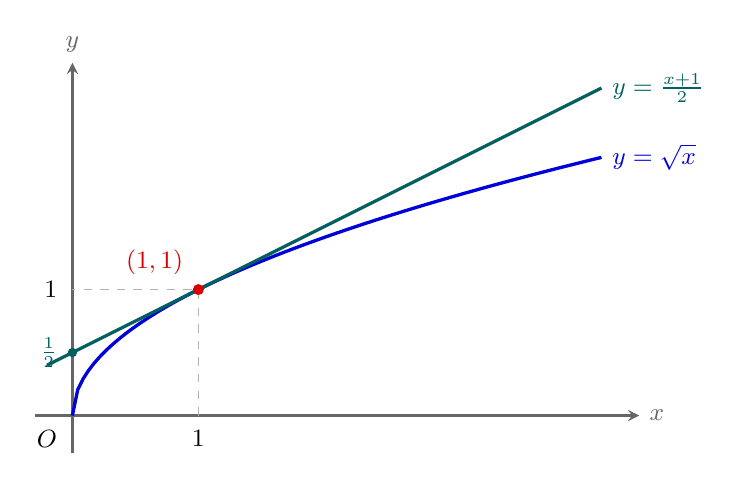
\begin{tikzpicture}[x=1.6cm, y=1.6cm, >=stealth,
    every node/.style={font=\small}]
    \draw[->, thick, gray!80!black] (-0.3, 0) -- (4.5, 0) node[right] {$x$};
    \draw[->, thick, gray!80!black] (0, -0.3) -- (0, 2.8) node[above] {$y$};
    \node[below left=2pt] at (0, 0) {$O$};

    % Curves
    \draw[line width=1.2pt, domain=0:4.2, samples=100, blue!85!black]
    plot (\x, {sqrt(\x)}) node[right] {$y = \sqrt{x}$};
    \draw[line width=1.2pt, domain=-0.2:4.2, teal!75!black]
    plot (\x, {0.5*(\x + 1)}) node[right] {$y = \frac{x+1}{2}$};

    % Tangent / contact point (1, 1)
    \draw[dashed, gray!60] (1, 0) -- (1, 1) -- (0, 1);
    \node[circle, fill=red!85!black, inner sep=1.4pt] at (1, 1) {};
    \node[above left=2pt, red!85!black] at (1, 1) {$(1, 1)$};

    % Intercepts and ticks
    \node[below=2pt] at (1, 0) {$1$};
    \node[left=2pt] at (0, 1) {$1$};
    \node[left=2pt, teal!75!black] at (0, 0.5) {$\frac{1}{2}$};
    \node[circle, fill=teal!75!black, inner sep=1.2pt] at (0, 0.5) {};
  \end{tikzpicture}
  \caption{$y = \dfrac{x+1}{2}$ と $y = \sqrt{x}$ のグラフ．}
  \label{fig:am_gm_graph}
\end{figure}

$x \ge 0$ より AM-GM不等式を用いて
\begin{align}
  \dfrac{x+1}{2} \ge \sqrt{x} \label{eq:1}
\end{align}
である．等号成立は$x=1$の時である．

\paragraph{(2)}

与えられた定積分を
\begin{align}
  A = \int_0^k\sqrt{x}{ \left( 1-\dfrac{x}{k} \right) }^kdx \label{eq:2}
\end{align}
とする．\cref{eq:1}から $[0, k]$ の時
\begin{align}
  \sqrt{x}\left(1 - \dfrac{x}{k}\right)^k \le \dfrac{1}{2}(x+1)\left(1 - \dfrac{x}{k}\right)^k
\end{align}
が成り立つ．等号成立は$x=1$の時のみだから，両辺同じ$[0,k]$で積分すると等号ははずせて
\begin{align}
  A < \dfrac{1}{2}\int_0^k (x+1)\left(1 - \dfrac{x}{k}\right)^k dx
\end{align}
となる．
$t = 1 - \dfrac{x}{k}$ とおくと $\dfrac{dt}{dx} = -\dfrac{1}{k}$，$x : 0 \to k$ で $t : 1 \to 0$ だから右辺の積分は
\begin{align}
  A &< \dfrac{1}{2} \int_1^0 \{1 + k(1-t)\} t^k \cdot (-k) dt \\
  &= \dfrac{1}{2} k \int_0^1 \{(1+k)t^k - k t^{k+1}\} dt \\
  &= \dfrac{1}{2} k \left[ t^{k+1} - \dfrac{k}{k+2} t^{k+2} \right]_0^1 \\
  &= \dfrac{1}{2} k \cdot \dfrac{2}{k+2} = \dfrac{1}{1 + 2/k} < 1 \quad (\because k \in \mathbb{N})
\end{align}
となって題意は示された．

\newpage

\end{document}
